% Options for packages loaded elsewhere
\PassOptionsToPackage{unicode}{hyperref}
\PassOptionsToPackage{hyphens}{url}
%
\documentclass[
]{article}
\usepackage{lmodern}
\usepackage{amssymb,amsmath}
\usepackage{ifxetex,ifluatex}
\ifnum 0\ifxetex 1\fi\ifluatex 1\fi=0 % if pdftex
  \usepackage[T1]{fontenc}
  \usepackage[utf8]{inputenc}
  \usepackage{textcomp} % provide euro and other symbols
\else % if luatex or xetex
  \usepackage{unicode-math}
  \defaultfontfeatures{Scale=MatchLowercase}
  \defaultfontfeatures[\rmfamily]{Ligatures=TeX,Scale=1}
\fi
% Use upquote if available, for straight quotes in verbatim environments
\IfFileExists{upquote.sty}{\usepackage{upquote}}{}
\IfFileExists{microtype.sty}{% use microtype if available
  \usepackage[]{microtype}
  \UseMicrotypeSet[protrusion]{basicmath} % disable protrusion for tt fonts
}{}
\makeatletter
\@ifundefined{KOMAClassName}{% if non-KOMA class
  \IfFileExists{parskip.sty}{%
    \usepackage{parskip}
  }{% else
    \setlength{\parindent}{0pt}
    \setlength{\parskip}{6pt plus 2pt minus 1pt}}
}{% if KOMA class
  \KOMAoptions{parskip=half}}
\makeatother
\usepackage{xcolor}
\usepackage{tikz}
\usetikzlibrary{arrows.meta}
\IfFileExists{xurl.sty}{\usepackage{xurl}}{} % add URL line breaks if available
\IfFileExists{bookmark.sty}{\usepackage{bookmark}}{\usepackage{hyperref}}
\hypersetup{
  hidelinks,
  pdfcreator={LaTeX via pandoc}}
\urlstyle{same} % disable monospaced font for URLs
\usepackage[margin=1in]{geometry}
\usepackage{longtable,booktabs}
% Correct order of tables after \paragraph or \subparagraph
\usepackage{etoolbox}
\makeatletter
\patchcmd\longtable{\par}{\if@noskipsec\mbox{}\fi\par}{}{}
\makeatother
% Allow footnotes in longtable head/foot
\IfFileExists{footnotehyper.sty}{\usepackage{footnotehyper}}{\usepackage{footnote}}
\makesavenoteenv{longtable}
\setlength{\emergencystretch}{3em} % prevent overfull lines
\providecommand{\tightlist}{%
  \setlength{\itemsep}{0pt}\setlength{\parskip}{0pt}}
\setcounter{secnumdepth}{-\maxdimen} % remove section numbering

\title{A Dynamic Programming Solution to Diff Alignment}
\author{Jonathan Simmonds}
\date{}

\begin{document}

\maketitle

\begin{abstract}
Diffs are commonly presented as patches - lines to add or remove from a
source file to result in a target file. For humans, this presentation
isn't always easy to follow - often diffs can be more intuitively
presented `side-by-side' - where the source file is shown on the left,
and the target file on the right. This presents an interesting problem
of deciding which changed lines to display together. This paper models
that decision as the shortest path through a weighted directed acyclic
graph of line-sequence prefixes. Removal, addition and pairing form the
graph's edges, and dynamic programming finds the minimum-cost,
order-preserving alignment. This gives a global optimisation for a given
cost model; explicit heuristics are defined to reject lines whose
character similarity would produce unintuitive matches. Cheap lower
bounds and a banded inner dynamic programme avoid unnecessary
edit-distance computation. The resulting method makes line pairing a
global decision while still leaving unrelated lines apart. An extension
is presented that uses the same pairwise alignment to give an alignment
for a three-way diff.
\end{abstract}

\hypertarget{problem-statement}{%
\section{Problem statement}\label{problem-statement}}

A line diff tells us which text survived and which text changed. That is
enough for a patch, but for a side-by-side presentation there's a
further choice to make: which changed line on the left belongs beside
which changed line on the right?

While that sounds like a small piece of layout work, it is a
surprisingly complex problem. A changed region with \(m\) lines on one
side and \(n\) on the other has one possible alignment for every path
through an \(m\) by \(n\) grid, and that number grows exponentially with
the size of the region. The choices also have visible consequences. A
poor alignment can make one edit look like several, or imply a
relationship between two lines which happen to contain similar
characters but say entirely different things.

What makes the problem particularly interesting is the split in the
solution. The graph and dynamic programme give an exact optimum for a
chosen cost model. The cost model captures the human judgement: when
does putting two lines together clarify the change?

Consider this small change:

\begin{longtable}[]{@{}p{0.46\linewidth}p{0.46\linewidth}@{}}
\toprule
Before & After\tabularnewline
\midrule
\endhead
\texttt{Kermit opens the show} &
\texttt{Tonight, Kermit opens the show}\tabularnewline
& \texttt{Statler heckles from the balcony}\tabularnewline
\texttt{Fozzie tells a joke} &
\texttt{Fozzie tells a terrible joke}\tabularnewline
\texttt{Gonzo fires the cannon} &
\texttt{Gonzo fires the cannon}\tabularnewline
\bottomrule
\end{longtable}

The first row is clearly one edited line. The empty cell belongs to
Statler's insertion. Fozzie's joke has been edited too, while Gonzo
provides an exact match at the end. Pairing by position gets this wrong
as soon as Statler starts heckling: every later line is shifted. Pairing
only exact matches also misses the relationships between the two edited
lines.

There is a less obvious failure at the other extreme. Given
\texttt{Miss\ Piggy\ enters\ gracefully} on one side and
\texttt{Animal\ attacks\ the\ drums} on the other, forcing the two lines
into alignment results in an unintuitive diff (and probably an argument
backstage). A good alignment would leave both lines unpaired.

The problem is therefore to find an order-preserving alignment of two
line sequences. Each output row consumes a line from the before
sequence, the after sequence, or both. It must consume every input line
exactly once, never change the order of either sequence, and should pair
lines only where doing so improves readability.

This is a global optimisation problem. A plausible match near the start
can steal a line from a much better match later, so a greedy walk is
insufficient. This naturally lends itself to a graph traversal problem.

\hypertarget{the-alignment-graph}{%
\section{The alignment graph}\label{the-alignment-graph}}

Let the before lines be

\[B = (b_1, b_2, \ldots, b_m)\]

and the after lines be

\[A = (a_1, a_2, \ldots, a_n).\]

Create a vertex \((i,j)\) for every pair of prefixes. The vertex means
that the first \(i\) before lines and the first \(j\) after lines have
been consumed. There are three possible outgoing steps:

\begin{longtable}[]{@{}lll@{}}
\toprule
Step & Edge & Meaning\tabularnewline
\midrule
\endhead
Remove & \((i,j) \rightarrow (i+1,j)\) & Put \(b_{i+1}\) on a row by
itself\tabularnewline
Add & \((i,j) \rightarrow (i,j+1)\) & Put \(a_{j+1}\) on a row by
itself\tabularnewline
Pair & \((i,j) \rightarrow (i+1,j+1)\) & Put the two next lines on one
row\tabularnewline
\bottomrule
\end{longtable}

For a small example, let the before side contain \texttt{Kermit} and
\texttt{Gonzo}, and the after side contain \texttt{Kermit!} and
\texttt{Animal}. The nodes use \texttt{K}, \texttt{G}, \texttt{K!} and
\texttt{A} as abbreviations for those lines. Each node shows the cheapest
partial alignment for the lines consumed at that point. The before and
after sides are separated by a vertical line; a dash means that the line
on the other side is unpaired. \(\varnothing\) represents the empty
alignment at the start.

\begin{figure}[ht]
\centering
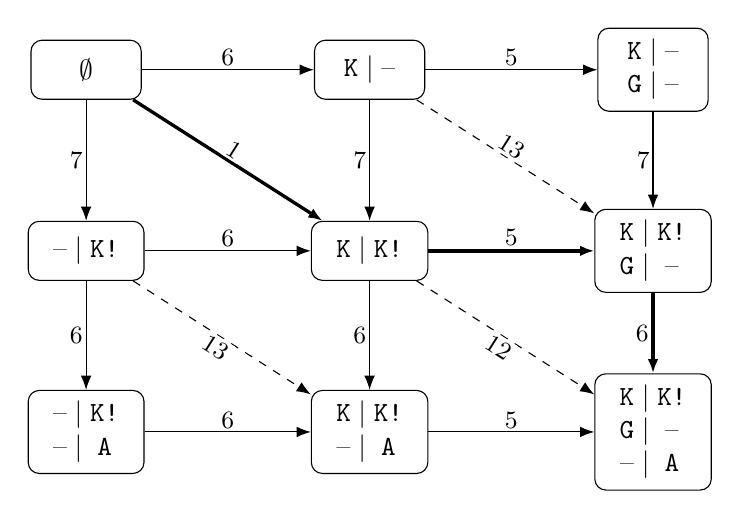
\begin{tikzpicture}[
  vertex/.style={draw, rounded corners, align=center, inner sep=3pt,
    minimum width=1.4cm, minimum height=0.75cm},
  edge/.style={-{Latex[length=1.8mm]}, thin},
  other pair/.style={edge, dashed},
  chosen/.style={edge, very thick},
  cost/.style={fill=white, inner sep=1pt, font=\small}
]
\node[vertex] (n00) at (0,4.6) {\(\varnothing\)};
\node[vertex] (n10) at (3.6,4.6) {\begin{tabular}{c@{\;|\;}c}
  \texttt{K} & --
\end{tabular}};
\node[vertex] (n20) at (7.2,4.6) {\begin{tabular}{c@{\;|\;}c}
  \texttt{K} & -- \\
  \texttt{G} & --
\end{tabular}};
\node[vertex] (n01) at (0,2.3) {\begin{tabular}{c@{\;|\;}c}
  -- & \texttt{K!}
\end{tabular}};
\node[vertex] (n11) at (3.6,2.3) {\begin{tabular}{c@{\;|\;}c}
  \texttt{K} & \texttt{K!}
\end{tabular}};
\node[vertex] (n21) at (7.2,2.3) {\begin{tabular}{c@{\;|\;}c}
  \texttt{K} & \texttt{K!} \\
  \texttt{G} & --
\end{tabular}};
\node[vertex] (n02) at (0,0) {\begin{tabular}{c@{\;|\;}c}
  -- & \texttt{K!} \\
  -- & \texttt{A}
\end{tabular}};
\node[vertex] (n12) at (3.6,0) {\begin{tabular}{c@{\;|\;}c}
  \texttt{K} & \texttt{K!} \\
  -- & \texttt{A}
\end{tabular}};
\node[vertex] (n22) at (7.2,0) {\begin{tabular}{c@{\;|\;}c}
  \texttt{K} & \texttt{K!} \\
  \texttt{G} & -- \\
  -- & \texttt{A}
\end{tabular}};

\draw[edge] (n00) -- node[cost, above] {6} (n10);
\draw[edge] (n10) -- node[cost, above] {5} (n20);
\draw[edge] (n01) -- node[cost, above] {6} (n11);
\draw[chosen] (n11) -- node[cost, above] {5} (n21);
\draw[edge] (n02) -- node[cost, above] {6} (n12);
\draw[edge] (n12) -- node[cost, above] {5} (n22);

\draw[edge] (n00) -- node[cost, left] {7} (n01);
\draw[edge] (n01) -- node[cost, left] {6} (n02);
\draw[edge] (n10) -- node[cost, left] {7} (n11);
\draw[edge] (n11) -- node[cost, left] {6} (n12);
\draw[edge] (n20) -- node[cost, left] {7} (n21);
\draw[chosen] (n21) -- node[cost, left] {6} (n22);

\draw[other pair] (n10) -- node[cost, above, sloped] {13} (n21);
\draw[other pair] (n01) -- node[cost, below, sloped] {13} (n12);
\draw[chosen] (n00) -- node[cost, above, sloped] {1} (n11);
\draw[other pair] (n11) -- node[cost, below, sloped] {12} (n22);
\end{tikzpicture}
\caption{Alignment graph for two lines on each side. Moving right
consumes a before line, moving down consumes an after line, and moving
diagonally pairs the two. Every edge is labelled with its cost; the
heavier edges form the shortest path.}
\label{fig:simple-alignment-graph}
\end{figure}

The chosen path pairs \texttt{Kermit} with \texttt{Kermit!} at a cost of
1, leaves \texttt{Gonzo} unpaired at a cost of 5, then does the same for
\texttt{Animal} at a cost of 6. Its total cost is therefore 12. The
other edges show the alternative alignments considered by the algorithm.

Every edge increases \(i+j\), so the graph is a directed acyclic graph
(DAG). More importantly, every legal alignment is a path from \((0,0)\)
to \((m,n)\), and every such path describes a legal alignment. The
alignment problem becomes a shortest-path problem once the edges have
costs.

This is the same grid structure which appears in global sequence
alignment {[}1{]}, string correction {[}2{]}, and file edit graphs
{[}3{]}. The items happen to be lines here, and the diagonal score asks
whether two lines look like revisions of one another.

\hypertarget{dynamic-programming-for-dag-traversal}{%
\section{Dynamic programming for DAG
traversal}\label{dynamic-programming-for-dag-traversal}}

Let \(D(i,j)\) be the minimum cost of aligning the two prefixes
(i.e.~their optimal alignment). Let \(|x|\) denote the number of
characters in line \(x\), and let \(p(x,y)\) be the cost of pairing two
lines. The shortest-path through this DAG is given by:

\[\begin{aligned}
D(i,j) = \min\{&D(i-1,j) + |b_i|,\\
               &D(i,j-1) + |a_j|,\\
               &D(i-1,j-1) + p(b_i,a_j)\}.
\end{aligned}\]

Its boundaries contain only gaps (unpaired lines):

\[D(i,0)=\sum_{k=1}^{i}|b_k|, \qquad
D(0,j)=\sum_{k=1}^{j}|a_k|.\]

By evaluating this table from top left to bottom right, we perform a
topological walk over the DAG. This dynamic programme relaxes each
cell's three incoming edges just once, and in doing so computes the
shortest-path.

The graph's construction results in the algorithm considering all legal
alignments without needing to enumerate them.

\hypertarget{scoring-an-alignment}{%
\section{Scoring an alignment}\label{scoring-an-alignment}}

The graph gives the cheapest alignment under the constraints presented
by the chosen cost model. This cost model represents the heuristic
choices which decide which pairs are useful to show, and which produce
too much noise. For example, the two strings \texttt{one\ dependable}
and \texttt{two\ unreliable} have a relatively low edit distance, but
differ in many positions and are unlikely to produce an intuitive
comparison.

Exact matches cost zero.

Treat a line left on its own as costing its character length. Thus,
leaving lines \(x\) and \(y\) unpaired costs

\[U(x,y)=|x|+|y|.\]

A pair should cost no more than leaving both lines apart. The current
implementation of \texttt{jiff}, favours pairing ties on the basis that
it gives a more compact representation.

For other pairs, the starting point is their Levenshtein distance
\(d(x,y)\), using unit-cost insertions, deletions and substitutions.
However, that distance cannot be used as the pair cost unconditionally:
consider two unrelated lines of the same length \(l\). Replacing every
character gives a distance no greater than \(l\), whereas leaving the
lines unpaired costs \(2l\). The shortest path would pair them, despite
there being no useful difference to show.

Let

\[M=\max(|x|,|y|), \qquad s=\min(|x|,|y|).\]

The implementation applies these rules:

\begin{enumerate}
\def\labelenumi{\arabic{enumi}.}
\tightlist
\item
  Identical lines always cost zero.
\item
  A pair is always rejected if \(M \geq 3s\).
\item
  A non-empty line which appears intact within the other is accepted
  with cost \(M-s\).
\item
  All other pairs are accepted only if \(d(x,y)<M/2\) with cost
  \(d(x,y)\).
\end{enumerate}

A rejected pair costs \(U(x,y)+1\). There is always a two-edge path
which leaves the lines unpaired for cost \(U(x,y)\), so the rejected
edge can never be chosen. Using a finite score means the
dynamic-programming calculation does not need a special case for
rejected pairs.

The ratio \(3\) and the \(1/2\) cutoff are choices about how readily to
pair lines. They come from the presentation rather than the graph and
are discussed further in
\protect\hyperlink{tuning-the-heuristics}{Tuning the heuristics}.

\hypertarget{avoiding-unnecessary-edit-distance-computation}{%
\section{Avoiding unnecessary edit-distance
computation}\label{avoiding-unnecessary-edit-distance-computation}}

Building the full outer table requires computing a score for every line
pair. However, the inner edit-distance calculation only needs to decide
whether the distance is at most the cutoff.

For the \(M/2\) threshold, the largest acceptable integer distance is

\[k=\left\lfloor\frac{M-1}{2}\right\rfloor.\]

Since it's only necessary to test whether \(d(x,y)\leq k\), larger
distances can be represented by \(k+1\). A few cheaper checks also
reduce the amount of text that needs to be examined:

\begin{itemize}
\tightlist
\item
  A matching prefix and suffix are removed. Keeping them is free, so
  this does not change the distance.
\item
  The difference in line lengths, \(M-s\), gives a lower bound on the
  distance.
\item
  If the two lines share \(S\) characters (including repeated
  characters), the multiset overlap is an upper bound on the number of
  characters they can share. Thus \(M-S\) gives a lower bound on edit
  distance.
\item
  The remaining edit-distance table only needs cells within \(k\) of its
  main diagonal. Anything outside that band already requires too many
  insertions or deletions and cannot be on the shortest-path.
\end{itemize}

It's also possible to store one row of the edit-distance table and reuse
that storage for the next candidate pair. These checks preserve the
result, they simply avoid work.

\hypertarget{walking-the-example}{%
\section{Walking the example}\label{walking-the-example}}

Consider the example from earlier again:

\begin{longtable}[]{@{}p{0.46\linewidth}p{0.46\linewidth}@{}}
\toprule
Before & After\tabularnewline
\midrule
\endhead
\texttt{Kermit opens the show} &
\texttt{Tonight, Kermit opens the show}\tabularnewline
& \texttt{Statler heckles from the balcony}\tabularnewline
\texttt{Fozzie tells a joke} &
\texttt{Fozzie tells a terrible joke}\tabularnewline
\texttt{Gonzo fires the cannon} &
\texttt{Gonzo fires the cannon}\tabularnewline
\bottomrule
\end{longtable}

The alignment follows this path:

\[(0,0)\rightarrow(1,1)\rightarrow(1,2)\rightarrow(2,3)
\rightarrow(3,4).\]

The first step pairs \texttt{Kermit\ opens\ the\ show} with
\texttt{Tonight,\ Kermit\ opens\ the\ show}. The original line appears
intact in the new one, giving a cost of nine. Statler's line is then
added on its own for a cost of 32. Fozzie's lines have edit distance
nine, which is below the cutoff of 13, and Gonzo's identical lines cost
zero. The complete path therefore costs

\[9+32+9+0=50.\]

The important choice is leaving Statler unpaired. Pairing him with
Fozzie would consume the Fozzie line from the before-side, rendering the
later pairing of the two similar lines unavailable. The dynamic
programme compares this with all other legal paths and chooses the
lowest total cost.

There can be several paths with the same cost. A pair wins a tie against
an unpaired line. Where add and remove are tied, the ordering is chosen
so removals appear first in the final output. This is an arbitrary
implementation choice but it makes the result repeatable and the
alignment consistent across the whole change.

\hypertarget{representing-the-graph-as-a-table}{%
\section{Representing the graph as a
table}\label{representing-the-graph-as-a-table}}

A naive implementation would build this DAG directly. Each possible
pair, addition or removal would be represented by a node containing its
score, best known cost and parent. Walking the nodes in topological
order would find the shortest-path (as described above), after which the
parent links can be followed to give the alignment.

However, the graph always has a fixed shape which can be exploited,
meaning it does not need to be stored as a collection of nodes. The
current implementation of \texttt{jiff} keeps two cost rows and one
operation value per cell for traceback. This performs the same
calculation without needing to store the graph nodes explicitly.

Choice of the cost function also needs some care. A segmented character
diff is simplest to reason about, but unnecessarily expensive. An
LCS-based distance, is better, but \texttt{jiff} ended up implementing
the bounded Levenshtein distance described above. An LCS could make
unrelated prose look similar by matching common letters and spaces
scattered through both lines. In \texttt{jiff}, the length and
character-frequency checks reject some candidates before calculating the
Levenshtein distance, further saving time.

\hypertarget{complexity}{%
\section{Complexity}\label{complexity}}

The line grid contains \((m+1)(n+1)\) cells, with constant work at each
cell once the pair score is known. Thus, traversing the grid takes
\(O(mn)\) time.

Let \(C_B\) and \(C_A\) be the total character counts on the two sides.
If every line pair requires a full edit-distance calculation, the work
sums to

\[\sum_i\sum_j |b_i||a_j|=C_BC_A.\]

This gives a worst-case time of \(O(mn+C_B+C_A+C_BC_A)\). The early
rejection checks significantly improve real-world performance, however
they don't change the bound.

Only the current and previous rows of costs are needed, using \(O(n)\)
space. The chosen operation at each cell takes another \(O(mn)\) bytes
and is used to recover the path. The inner edit-distance calculation
also keeps a single row, sized to the shorter of the two lines.

\hypertarget{three-way-alignment}{%
\section{Three-way alignment}\label{three-way-alignment}}

This algorithm can be applied to three-way diffs, as often encountered
when merging changes (combining two independent changes targeting the
same regions of the same file). This can be computed by treating the
middle input as the base; aligning left/base and base/right
independently; then joining the results following the base's line index.
Outer-only lines attach to the relevant base line, as in a standard
two-way alignment. Insertions at the same line may share a display row,
but that does not necessarily mean both sides match. This gives two
separate pairwise alignments joined through the base, rather than an
optimal three-way cost model. In addition to being simpler to implement,
this tends to produce a more intuitive presentation as most comparisons
in a three-way diff are relative to the base rather than between each
side.

\hypertarget{limits}{%
\section{Limits}\label{limits}}

The alignment preserves line order, an important constraint for making
an intuitive diff. This means moved blocks are shown as a removal and an
addition.

Line similarity is based on characters rather than syntax. A
syntax-aware pair score could be substituted without changing the outer
graph, but it would make different mistakes and cost more to calculate.

Unpaired lines are scored independently. There is no extra cost for
starting a new block of additions or removals, so the scoring does not
distinguish between one continuous block and the same number of unpaired
lines spread across several blocks. Supporting that distinction would
require the table to keep separate costs for paths ending in an
addition, a removal or a pairing.

\hypertarget{tuning-the-heuristics}{%
\section{Tuning the heuristics}\label{tuning-the-heuristics}}

The choices that affect the output are:

\begin{itemize}
\tightlist
\item
  The maximum line-length ratio.

  \begin{itemize}
  \tightlist
  \item
    The current rule rejects a pair when \(M\geq3s\). Reducing the
    multiplier rejects more uneven pairs; increasing it allows shorter
    lines to be paired with much longer ones.
  \end{itemize}
\item
  The edit-distance cutoff.

  \begin{itemize}
  \tightlist
  \item
    The current rule is \(d(x,y)<M/2\). A smaller fraction gives fewer
    pairings; a larger one accepts lines with less in common.
  \end{itemize}
\item
  The contiguous-line exception.

  \begin{itemize}
  \tightlist
  \item
    A shorter line found intact inside the longer one bypasses the
    edit-distance cutoff (although it must still pass the length check).
    Removing this exception would reject large prefix or suffix
    additions.
  \end{itemize}
\item
  The cost model.

  \begin{itemize}
  \tightlist
  \item
    Unpaired lines cost their character count and each of the three edit
    operations cost one. These could be weighted differently, for
    example if whitespace changes should count less than non-whitespace
    changes, or if substitutions should cost more than
    additions/removals.
  \end{itemize}
\item
  Tie-breaking.

  \begin{itemize}
  \tightlist
  \item
    Pairing currently wins an equal-cost choice. Preferring separation
    would make the output slightly more conservative.
  \end{itemize}
\end{itemize}

These heuristics were tuned by a non-scientific and objective process of
using the tool and collecting feedback. There is no labelled corpus of
examples or large A-B tested study to inform the decision, so \(3\) and
\(1/2\) remain somewhat arbitrary judgement calls. In real-world use,
false pair is usually more distracting than a missed pairing, which is
why the heuristics presented above currently bias conservatively.

The other techniques described: prefix and suffix removal, the
character-frequency lower bound and the banded edit-distance calculation
are not heuristics. They are safe optimisations on the method that don't
alter the output.

\hypertarget{references}{%
\section{References}\label{references}}

\begin{enumerate}
\def\labelenumi{\arabic{enumi}.}
\tightlist
\item
  Saul B. Needleman and Christian D. Wunsch, ``A general method
  applicable to the search for similarities in the amino acid sequence
  of two proteins'', \emph{Journal of Molecular Biology} 48(3),
  443--453, 1970. \url{https://doi.org/10.1016/0022-2836(70)90057-4}
\item
  Robert A. Wagner and Michael J. Fischer, ``The string-to-string
  correction problem'', \emph{Journal of the ACM} 21(1), 168--173, 1974.
  \url{https://doi.org/10.1145/321796.321811}
\item
  Eugene W. Myers, ``An O(ND) difference algorithm and its variations'',
  \emph{Algorithmica} 1, 251--266, 1986.
  \url{https://doi.org/10.1007/BF01840446}
\end{enumerate}

\end{document}
